\documentclass{article}
\usepackage[utf8]{inputenc}

\title{Desenvolvimento de metamodelo para predição de carga térmica de ar condicionado em edificações residenciais unifamiliares.}
\author{Marcelo Salles Olinger}
\date{Março 2021}

\usepackage[round]{natbib}
\usepackage{graphicx}

\usepackage[acronym]{glossaries}
% Abreviaturas
\newacronym{vn}{VN}{ventilação natural}
\newacronym{iea}{IEA}{Agência Internacional de Energia}
\newacronym{aivc}{AIVC}{\textit{Air Infiltration and Ventilation Centre}}
\newacronym{hvac}{HVAC}{\textit{heating, ventilating and air conditioning}}
\newacronym{pmv}{PMV}{voto predito médio}
\newacronym{ann}{RNA}{redes neurais artificiais}
\newacronym{svm}{MVS}{máquinas de vetores de suporte}
\newacronym{cfd}{CFD}{\textit{Computer Fluid Dynamics}}
\newacronym{afn}{AFN}{\textit{Airflow Network}}
\newacronym{ct}{CT}{capacidade térmica}
\newacronym{cp}{$C_p$}{coeficientes de pressão}
\newacronym{cq}{$C_Q$}{coeficiente de fluxo mássico de ar}
\newacronym{cpeq}{$C_{p,eq}$}{coeficiente de pressão equivalente}
\newacronym{cd}{$C_d$}{coeficiente de descarga}
\newacronym{tpu}{TPU}{Universidade Politécnica de Tóquio}
\newacronym{paf}{PAF}{percentual de abertura na fachada}
\newacronym{fs}{FS}{fator solar}
\newacronym{as}{AS}{análise de sensibilidade}
\newacronym{ehf}{EHF}{fração de horas de desconforto por calor}
\newacronym{ach}{ACH}{trocas de ar por hora}
\newacronym{rmse}{RMSE}{raiz quadrada do erro quadrático médio}
\newacronym{nrmse}{NRMSE}{raiz quadrada do erro quadrático médio normalizada}
\newacronym{r2}{R$^2$}{coeficiente de determinação}
\newacronym{abse}{MAE}{erro absoluto médio}
\newacronym{ae95}{AE95}{erro absoluto do 95º percentil}
\newacronym{ma}{MA}{método analítico}
\newacronym{inic}{INI-C}{Proposta de Instrução Normativa do Inmetro para a Classe de Eficiência Energética de Edificações Comerciais, de Serviços e Públicas}
\newacronym{gboost}{GBoost}{Gradient Boost}

\usepackage{hyperref}

\begin{document}

\maketitle

\section{Introdução}

De acordo com a \acrfull{iea} \citep{IEA2018a}, no ano de 2017 o setor de edificações representou mais de 30\% do consumo final total de energia no mundo. 
O relatória da \citet{IEA2018} aponta que a demanda por energia destinada ao resfriamento de ar em edificações mais que triplicou do ano de 1990 a 2016 e, se não houver mudanças no cenário atual, estima-se que essa demanda mais que triplicará até o ano de 2050, representando 37\% do aumento no consumo de eletricidade em edificações. 
O potencial de aumento na demanda por energia destinada ao resfriamento de ar em países de clima quente é ainda mais expressivo. Das 2,8 bilhões de pessoas que vivem nas partes mais quentes do mundo hoje, apenas 8\% possuem sistema de condicionamento de ar \citep{IEA2018}. No Brasil, a parcela do resfriamento de ar nas cargas de pico das redes elétricas em 2016 correspondia a 7,6\% do total, e a estimativa, considerando-se o cenário base, é de que essa parcela represente 30,8\% da carga de pico até o ano de 2050 \citep{IEA2018}. 

Para que o conforto térmico dos usuários seja garantido sem um consumo significativo de energia, é importante entender como ocorrem as variações térmicas em um edifício antes de construí-lo. Análises durante os estágios iniciais de projeto de uma edificação com \acrlong{vn} apontam decisões fundamentais para o desempenho térmico. No estágio inicial de projeto, o potencial de otimização é significativo, e nesta etapa qualquer estimativa do conforto e desempenho energético da edificação pode refletir nas tomadas de decisão \citep{Belleri2014, Roetzel2014}.

O método mais avançado de se estimar o desempenho termoenergético de edificações atualmente é por meio de simulações computacionais, que utilizam modelos baseados em equações físicas de transferência de calor, seguindo os princípios da conservação de energia.
No entanto, esse processo exige o conhecimento técnico de um especialista, pois simulações termoenergéticas dinâmicas requerem modelos detalhados e enfrentam diversos problemas, associados principalmente a informações necessárias para dados de entrada do modelo processado \citep{Corgnati2013}. No contexto brasileiro, a análise do desempenho térmico de edificações por meio de simulações computacionais é uma medida relevante, pois, assim como em outros países em desenvolvimento, a falta de acessibilidade a dados relacionados a padrões de consumo de energia e atributos físicos e operacionais de edifícios de escritório dificulta as análises a partir de bancos de dados \citep{Alves2018}. Uma alternativa para contornar essas questões é o desenvolvimento de modelos a partir de simulações computacionais, os metamodelos. Por meio de metamodelos é possível se obter resultados próximos aos de simulações complexas de desempenho energético.

Metamodelos para eficiência energética de edificações podem ser desenvolvidos a partir de diferentes métodos \citep{Ostergard2018}. A solução mais apropriada depende do contexto e propósitos de cada aplicação.
\citet{Versage2015} foi capaz de estimar as cargas térmicas de edificações comerciais através de diferentes métodos de metamodelagem.
\citet{Melo2016} desenvolveram um modelo de \acrlong{ann} para estimar graus hora de resfriamento e cargas térmicas de aquecimento e resfriamento em edificações residenciais.
O desenvolvimento de um metamodelo de máquina de vetores de suporte capaz de estimar conforto térmico em edificações comerciais foi proposto por \citet{Rackes2016}. 

O consumo de energia para resfriamento de edificações é expressivo no mundo, e a expectativa é de que a demanda por energia continue crescendo nas próximas décadas, principalmente em países de climas quentes.
Neste contexto, o uso de técnicas construtivas que minimizam a necessidade de ar condicionado, por meio de componentes construtivos específicos ou pelo uso de \acrlong{vn}, apresentam-se como uma solução para mitigar o consumo de energia.
Entretanto, o desempenho térmico das edificações apresenta fenômenos termofísicos complexos, fazendo com que estimativas de conforto térmico devam ser consideradas preferencialmente desde as etapas iniciais de projeto. 	
Na busca por uma ferramenta capaz de auxiliar projetistas de maneira rápida e simples, surge a possibilidade de utilizar-se metamodelos.
Portanto, este trabalho apresenta uma comparação entre duas abordagens de aprendizado de máquina para o desenvolvimento de um metamodelo capaz de estimar a carga térmica de resfriamento em edificações unifamiliares.

\section{Revisão}
%%%%%%%%%%%%%%%%%%%%%%%%%%%%%%%%%%%%%%%%%%%%%%%%%%%%%%%%%%

Projetistas encontram dificuldades no uso de ferramentas de simulação de desempenho termoenergético em edificações, que podem não ser compatíveis com suas necessidades e métodos de trabalho. Por isso, autores como \citet{Picco2014a} propõem simplificar a descrição do edifício e converter um modelo detalhado em um modelo simplificado, com apenas um número limitado de entradas. Apesar das margens de erro de cerca de 15\% na estimativa de cargas térmicas anuais de aquecimento e resfriamento, os autores observaram que simplificações no modelo podem auxiliar em estágios iniciais de projeto, quando certas características no projeto do edifício ainda não estão bem definidas.

Além das simplificações nos modelos baseados em equações físicas, é possível desenvolver modelos baseados em funções estatísticas, que deduzem esses comportamentos. Modelos estatísticos funcionam apenas com entradas e saídas, sem correlacionar causa e efeito, mas têm maior agilidade. Para adaptar as principais funcionalidades de ambos os modelos, existem os metamodelos.

Metamodelos baseados em aprendizado automático são funções matemáticas que, aplicadas a uma quantidade significativa de dados, conseguem identificar padrões ocultos e prever o que poderá ocorrer. De acordo com  \citet{Zhao2012}, os métodos de aprendizado automático mais utilizados para predição de desempenho energético de edificações são \acrfull{ann} e \acrfull{svm}. Esses modelos são altamente eficazes na solução de problemas não-lineares, e podem oferecer predições altamente acuradas, desde que as definições do modelo e parâmetros estabelecidos estejam definidos adequadamente. Modelos de \acrshort{ann} já foram usados para analisar vários tipos de consumo de energia em edificações em diversas condições, como em cargas de aquecimento e resfriamento, consumo de eletricidade, operação e otimização de componentes, e estimativa de parâmetros de uso. O uso de \acrshort{svm} vem crescendo em pesquisas e indústria. Em muitos casos as \acrshort{svm} mostram performances superiores às das \acrshort{ann}, mesmo com pequena quantidade de dados para treinamento.

\citet{YIGIT2021} desenvolveu um metamodelo utilizando \textit{Gradient Boosting Machine} (GBM), por meio da biblioteca Sklearn, para estimar cargas de resfriamento e aquecimento em edifícios residenciais na Turquia. 
Segundo o autor, modelos de GBM são baseados em modelos de árvore de decisão, e já demonstraram alto desempenho e flexibilidade em diversas áreas. 
Esses modelos são capazes de de lidar com base de dados com grande quantidade de variáveis, discretas e/ou contínuas sem necessidade de pre-processamento dos dados. 
O método do GBM possibilita o desenvolvimento de metamodelos robustos independentemente do número de parâmetros ou tipo de parâmetros. 
A inclusão de parâmetros com baixa influência nas variáveis dependentes também não compromete a acurácia do modelo. 
Destaca-se a importância na escolha dos hiperparâmetros para garantir melhor desempenho dos modelos.
O metamodelo desenvolvido no trabalho de \citet{YIGIT2021} foi aplicado em um algorítimo de otimização, para encontrar os tipos de envoltórias mais apropriados para minimizar os consumo energético. Os resultados mostraram que a utilização do sistema de otimização pode trazer soluções de projeto com maior eficiência energética e baixo custo. Além disso, o aumento no custo da envoltória da edificação pode reduzir a o conusmo de energia em até 10\%.
No entanto, o autor comenta que a implementação de GBM em problemas de otimização de energia em edificações ainda é limitada.

\citet{Versage2015} desenvolveu um metamodelo para estimar a carga integrada anual de energia de refrigeração para avaliação de desempenho energético de edificações condicionadas artificialmente através do desempenho individual de suas zonas térmicas. Foi desenvolvida uma base de dados de aproximadamente 1,29 milhões de casos simulados, com parâmetros construtivos variados, para o clima de Florianópolis. Uma amostra dos dados foi adotada para a elaboração de metamodelos com as técnicas de regressão linear múltipla, regressão adaptativa multivariada por \textit{splines}, processo gaussiano, máquina de vetores de suporte, \textit{random forest} e \acrlong{ann}. Para avaliar e comparar os metamodelos, quatro índices de desempenho foram escolhidos: tempo de treinamento, coeficiente de determinação (\acrshort{r2}), \acrshort{rmse} e \acrfull{nrmse}. O metamodelo de \acrshort{ann} obteve o melhor desempenho entre os testados. A rede neural artificial treinada com 1\% dos casos do banco de dados, e com 72 nós na camada interna, obteve o melhor desempenho global, e foi capaz de reproduzir resultados com erros menores que 10\% para 99,2\% dos casos. O metamodelo elaborado a partir de \acrshort{svm} obteve o pior desempenho. Porém, o autor destaca que outras configurações e tratamentos dos dados poderiam mudar o desempenho dos metamodelos avaliados.

De acordo com a bibliografia levantada, observa-se que diferentes métodos de aprendizagem automática podem ser utilizados para o desenvolvimento de metamodelos relacionados à eficiência energética em edificações. 
Não há uma regra para a escolha do método, e a comparação entre o desempenho de metamodelos desenvolvidos por diferentes abordagens de aprendizado de máquina  podem depender da configuração dos hiperparâmetros, ou até mesmo de características específicas do banco de dados utilizados, como os parâmetros de entrada e de saída considerados.
Portanto, pode ser pertinente considerar o uso de mais de um tipo de máquina de aprendizado na busca pelo método mais adequado.

\section{Método} %%%%%%%%%%%%%%%%%%%%%%%%%%%%%%%%%%%%%%%%%%%%%%%%%%%%%%%%%%%%%%

Este trabalho utilizou um \href{https://drive.google.com/uc?export=download&id=1XROGI9ZaUX711MjWiyEMv4U84lZFUcGW}{banco de dados} composto por análises termoenergéticas de edificações, para desenvolver metamodelos por duas abordagens: \acrfull{ann} e \textit{Gradient Boosting Machine} (GBM).
Os desempenho dos metamodelos entre as duas abordagens foi comparado, assim como questões específicas do desenvolvimento de cada uma foram discutidas.
Os treinamentos dos modelos foram conduzidos utilizando-se 19 processos paralelos em uma máquina com processador Intel Xeon de 3,30 GHz.

O código utilizado para o desenvolvimento do metamodelo está disponível na \href{https://github.com/marcelosalles}{conta do \texttt{github} do autor}, no endereço:

\url{https://github.com/marcelosalles/disciplina-machine-learning.git}

\subsection{O banco de dados}

O \href{https://drive.google.com/uc?export=download&id=1XROGI9ZaUX711MjWiyEMv4U84lZFUcGW}{banco de dados (link)} utilizados para este trabalho é composto por análises termoenergéticas de edificações, simuladas por meio do programa computacional EnergyPlus \citep{EnergyPlus2018}. 
O dado de saída das simulações é a carga térmica de ar condicionado necessária para manter a temperatura do ar nas zonas térmicas ocupadas da edificação entre 21 $^{\circ}$C e 23 $^{\circ}$C.
As simulações foram baseadas em um modelo base (Figura \ref{fig:modelo}) de uma edificação unifamiliar de interesse social do trabalho de \citet{TRIANA2018}, que teve diversas características construtivas variadas, relacionadas à geometria da envoltória e das janelas, assim como componentes construtivos. 

\begin{figure}[h]
	\caption{Modelo base das simulações.} % of{figure}
	\label{fig:modelo}
	\centering
	\begin{minipage}{.5\textwidth}
		\centering
		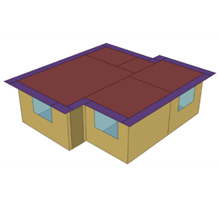
\includegraphics[width=\linewidth]{modelo_casinha.png}
	\end{minipage}%
	\begin{minipage}{.3\textwidth}
		\centering
		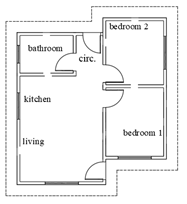
\includegraphics[width=\linewidth]{planta_casinha.png}
	\end{minipage}%
\end{figure}

A Tabela \ref{table:quantvars} apresenta os parâmetros de valores quantitativos, com os valores máximos e mínimos considerados na amostragem. 
A Tabela \ref{table:qualivars} apresenta as variações dos parâmetros qualitativos. Apesar de serem qualitativas, as variáveis são representadas no banco de dados por números inteiros, variando de 1 a 6 para a parede, 1 a 4 para a cobertura, e 0 ou 1 para venezianas e espelhamento da geometria.

\begin{table}[h!]
	\centering
	\caption{Parâmetros quantitativos considerados na base de dados.}
	\label{table:quantvars}
	\begin{tabular}{|c |c |c |}
		\hline
		\textbf{Parâmetro} & \textbf{Valor mínimo} & \textbf{Valor máximo} \\
		\hline
		Área [$m^{2}$] & 48 & 152 \\
		\hline
		Razão entre eixos [-] & 0,47 & 2,03 \\
		\hline
		Pé-direito [$m$] & 2,48 & 3,52 \\
		\hline
		Azimute [$graus$] & 0 & 360 \\
		\hline
		Absortância das paredes [-] & 0,19 & 0,81 \\
		\hline
		Absortância da cobertura [-] & 0,19 & 0,81 \\
		\hline
		PAF* da sala [-] & 0,19 & 0,81 \\
		\hline
		PAF* dos dormitórios [-] &  0,19 & 0,81 \\
		\hline
		Transmitância do vidro [$W/m^{2}K$] & 2,74 & 5,76 \\
		\hline
		Fator solar do vidro [-] & 0,21 & 0,88 \\
		\hline
		Fator de abertura da janela [-] & 0,39 & 0,91 \\
		\hline
		Temperatura média anual [$^{\circ}C$] & 10,8 & 28,2 \\
		\hline 
	\end{tabular}\\
	\small{* PAF = Percentual de Abertura na Fachada}
\end{table}

\begin{table}[h!]
	\centering
	\caption{Parâmetros qualitativos considerados na base de dados.}
	\label{table:qualivars}
	\begin{tabular}{|c |l |}
		\hline
		\textbf{Parâmetro} & \textbf{Valores} \\
		\hline
		{} & Concreto \\
		{} & Concreto + EPS \\
		{} & \textit{Steel frame} \vspace{-6pt} \\
		Parede & {} \vspace{-6pt}\\
		{} & Tijolo maciço (10 cm) \\
		{} & Tijolo maciço (20 cm) \\
		{} & Tijolo vazado \\
		\hline
		{} & Telha de fibrocimento + laje de concreto \\
		{} & Telha de fibrocimento + lã de vidro (2,5 cm)+ laje de concreto \vspace{-6pt} \\
		Cobertura & {} \vspace{-6pt}\\
		{} & Telha de fibrocimento + lã de vidro (5,0 cm)+ laje de concreto \\
		{} & Telha de fibrocimento + laje de concreto + gesso\\
		\hline
		Veneziana & Sim / Não \\
		\hline
		Geometria espelhada & Sim / Não \\
		\hline 
	\end{tabular}\\
% 	\small{}
\end{table}

Os 46.696 casos do banco de dados foram amostrados pelo método de Sobol \citep{Sobol1993}, método de amostragem quasi-randômico que garante melhor distribuição de casos no hiperespaço. As distribuições das variáveis de entrada foram uniformes.
A Figura \ref{fig:db_hist} apresenta a distribuição de ocorrência das variáveis independentes, assim como da variável dependente.
O único parâmetro de entrada que não apresenta distribuição uniforme é a Temperatura média anual, pois apesar de a temperatura média ter sido amostrada uniformemente para valores entre 10,8 $^{\circ}C$ e 28,2 $^{\circ}C$, na base de arquivos climáticos do Brasil não existem cidades com temperaturas médias anuais entre 10,8 $^{\circ}C$ e 13,6 $^{\circ}C$, e há apenas três cidades com temperaturas médias anuais entre 13,6 $^{\circ}C$ e 15,3 $^{\circ}C$. 
Como consequência, os casos amostrados com temperaturas nessas faixas foram simulados utilizando-se os arquivos climáticos com as temperaturas médias anuais mais próximas do valor amostrado.
O parâmetro de saída, Carga térmica de ar condicionado, teve uma distribuição não uniforme, que variou entre 0 e 235 kWh/m²ano, com média igual a 53 kWh/m²ano e mediana igual a 43 kWh/m²ano. 

\begin{figure}[h!]
	\caption{Distribuições de ocorrência dos parâmetros de entrada.} % of{figure}
	\label{fig:db_hist}
	\centering
	\begin{minipage}{.33\textwidth}
		\centering
		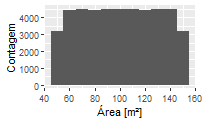
\includegraphics[width=\linewidth]{plot_area.png}
	\end{minipage}%
	\begin{minipage}{.33\textwidth}
		\centering
		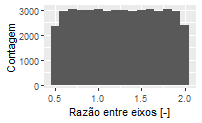
\includegraphics[width=\linewidth]{plot_ratio.png}
	\end{minipage}%
	\begin{minipage}{.33\textwidth}
		\centering
		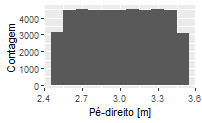
\includegraphics[width=\linewidth]{plot_height.png}
	\end{minipage}
	\centering
	\begin{minipage}{.33\textwidth}
		\centering
		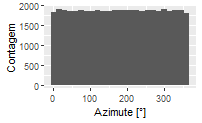
\includegraphics[width=\linewidth]{plot_azimute.png}
	\end{minipage}%
	\begin{minipage}{.33\textwidth}
		\centering
		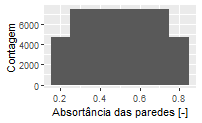
\includegraphics[width=\linewidth]{plot_abs_wall.png}
	\end{minipage}%
	\begin{minipage}{.33\textwidth}
		\centering
		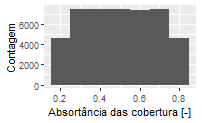
\includegraphics[width=\linewidth]{plot_abs_roof.png}
	\end{minipage}
	\centering
	\begin{minipage}{.33\textwidth}
		\centering
		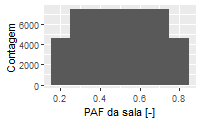
\includegraphics[width=\linewidth]{plot_wwr_living.png}
	\end{minipage}%
	\begin{minipage}{.33\textwidth}
		\centering
		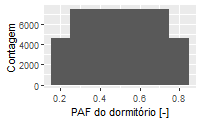
\includegraphics[width=\linewidth]{plot_wwr_bedroom.png}
	\end{minipage}%
	%\end{figure}
	%\begin{figure}
	%	\ContinuedFloat
	%	\caption[]{\textit{Continuação}} % {figure}
	%	\centering	
	\begin{minipage}{.33\textwidth}
		\centering
		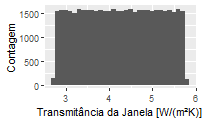
\includegraphics[width=\linewidth]{plot_window_u.png}
	\end{minipage}
	\centering
	\begin{minipage}{.33\textwidth}
		\centering
		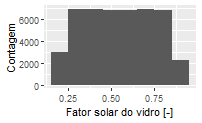
\includegraphics[width=\linewidth]{plot_shgc.png}
	\end{minipage}%
	\begin{minipage}{.33\textwidth}
		\centering
		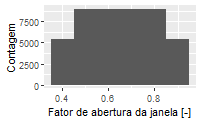
\includegraphics[width=\linewidth]{plot_open_fac.png}
	\end{minipage}%
	\begin{minipage}{.33\textwidth}
		\centering
		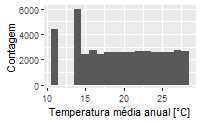
\includegraphics[width=\linewidth]{plot_DBT.png}
	\end{minipage}
	\centering	
	\begin{minipage}{.33\textwidth}
		\centering
		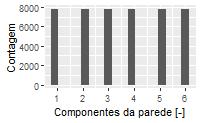
\includegraphics[width=\linewidth]{plot_shell_wall.png}
	\end{minipage}%
	\begin{minipage}{.33\textwidth}
		\centering
		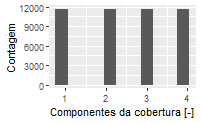
\includegraphics[width=\linewidth]{plot_shell_roof.png}
	\end{minipage}%
	\begin{minipage}{.33\textwidth}
		\centering
		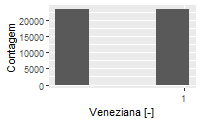
\includegraphics[width=\linewidth]{plot_blind.png}
	\end{minipage}
	%	\centering
	\begin{minipage}{.33\textwidth}
		%		\centering
		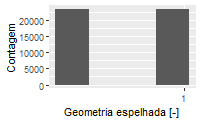
\includegraphics[width=\linewidth]{plot_mirror.png}
	\end{minipage}
	\begin{minipage}{.33\textwidth}
		%		\centering
		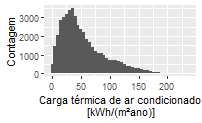
\includegraphics[width=\linewidth]{plot_cgtt.png}
	\end{minipage}
\end{figure}

\subsection{Desenvolvimento da rede neural artificial}

O metamodelo de \acrshort{ann} foi desenvolvido utilizando-se a biblioteca Sklearn \citep{scikit-learn}, disponibilizada para \citet{Python}.
As variáveis quantitativas foram padronizadas calculando-se o \textit{z-score}, de acordo com a Equação \ref{eq:zscore}, para que todos os parâmetros tivessem a mesma ordem de grandeza.

\begin{equation}\label{eq:zscore}
Z = \frac{x-\mu}{\sigma}
\end{equation}

Onde $Z$ é igual ao novo valor considerado para a variável $x$; $\mu$ é a média dos valores da variável considerada; e $\sigma$ é o valor do desvio padrão da variável considerada.

As variáveis qualitativas foram transformadas em \textit{dummy variables}, portanto cada coluna de parâmetros de valores qualitativos no \textit{dataframe} foi substituída por novas colunas. Essas novas colunas representam os diferentes valores considerados para o parâmetro de valores qualitativos. 
Assim, para cada linha do \textit{dataframe} é atribuído o valor 1 para a coluna referente ao valor considerado para o parâmetro qualitativo naquela linha, e o valor 0 para as demais colunas, referentes aos demais valores possíveis para aquele parâmetro.
O número de novas colunas introduzidas para substituir a coluna original do parâmetro depende da quantidade de valores únicos. O número de colunas introduzidas é igual ao número de valores únicos do parâmetro menos 1, pois para indicar que um caso possui o valor relacionado à variável sem coluna correspondente, basta considerar o valor 0 em todas as outras colunas referentes àquele parâmetro.

É importante também observar os hiperparâmetros (parâmetros relacionados ao processo de aprendizagem automática) escolhidos no desenvolvimento do metamodelo, que influenciam na acurácia dos resultados obtidos.
Portanto, uma busca por \textit{grid} foi conduzida, a fim de se encontrar a melhor combinação de hiperparâmetros.
Os hiperparâmetros variados foram:

\begin{itemize}
    \item \texttt{hidden\_layer\_sizes}: o número de camadas ocultas e número de nós nessas camadas;
    \item \texttt{activation}: a função de ativação utilizada;
    \item \texttt{batch\_size}: o número de casos utilizados em cada iteração no processo de otimização estocástica;
    \item \texttt{learning\_rate\_init}: a taxa de aprendizagem;
    \item \texttt{tol}: valor mínimo de redução da função perda ao longo de um número de iterações especificado (para este trabalho, o número de iterações especificado foi igual a 10).
\end{itemize}

Os valores aplicados no \textit{grid} para buscar a combinação ótima de hiperparâmetros estão apresentados na Tabela \ref{table:hiperparemtrosann}

\begin{table}[!htb]
	\centering
	\caption{Hiperparâmetros considerados na busca por \textit{grid} da rede neural artificial.}
	\label{table:hiperparemtrosann}
	\begin{tabular}{|c |c |}
		\hline
		\textbf{Hiperparâmetro} & \textbf{Valores} \\
		\hline
		\texttt{hidden\_layer\_sizes} & 32 e 64; 64 e 128; 32, 64 e 128 \\
		\hline
		\texttt{activation} & \texttt{logistic}; \texttt{relu} \\
		\hline
		\texttt{batch\_size} & 32; 64; 128 \\
		\hline
		\texttt{learning\_rate\_init} & 0,005; 0,01; 0,05  \\
		\hline
		\texttt{tol} & 0,0001; 0,0005; 0,00005 \\
		\hline
	\end{tabular}\\
% 	\small{}
\end{table}

Antes da etapa de treinamento do metamodelo a amostra foi dividida em um \textit{dataframe} para treinamento, com 90\% dos casos, e um \textit{dataframe} para teste, com os 10\% restante dos casos.
O indicador de desempenho utilizado para comparar os diferentes modelos gerados pelo \textit{grid} foi a média da pontuação da validação cruzada (\textit{cross-validation score}).
O modelo de \acrshort{ann} com a melhor pontuação na etapa de treinamento foi escolhido para ter seu desempenho analisado com as amostras de treinamento e de teste. 
Os indicadores de acurácia do metamodelo final foram: o \acrfull{r2}, o \acrfull{rmse}, o erro absoluto médio (MAE) e o \acrfull{ae95}.

\subsection{Desenvolvimento do \textit{Gradient Boosting Machine}}%%%%%%%%%%%%%%%%%%%%%%%%%%%%%%%%%%%%%%%%%%%%%%%%%%%%%%%%%%%%%%%%

O metamodelo de \textit{Gradient Boosting Machine} (GBM) também foi desenvolvido utilizando-se a biblioteca Sklearn \citep{scikit-learn}, disponibilizada para \citet{Python}.
Como essa abordagem não exige pré-processamento dos dados, não houve padronização, nem transformação de variáveis qualitativas em diversas colunas de \textit{dummy variables}. 

Os hiperparâmetros também foram definidos a partir de uma busca por \textit{grid}.
Os hiperparâmetros variados foram:

\begin{itemize}
    \item \texttt{n\_estimators}: o número de estimadores, ou árvores;
    \item \texttt{max\_depth}: o número máximo de nós em cada árvore;
    \item \texttt{min\_samples\_split}: o número mínimo de casos requeridos em uma folha de um nó;
    \item \texttt{loss}: a função perda. \texttt{ls} refere-se à regressão dos mínimos quadrados, \texttt{lad} refere-se à função do mínimo desvio absoluto, e \texttt{huber} refere-se um método que combina os dois anteriores;
    \item \texttt{learning\_rate}: a taxa de aprendizagem.
\end{itemize}

Os valores aplicados no \textit{grid} para buscar a combinação ótima de hiperparâmetros para o GBM estão apresentados na Tabela \ref{table:hiperparemtros}

\begin{table}[!htb]
	\centering
	\caption{Hiperparâmetros considerados na busca por \textit{grid} do GBM.}
	\label{table:hiperparemtros}
	\begin{tabular}{|c |c |}
		\hline
		\textbf{Hiperparâmetro} & \textbf{Valores} \\
		\hline
		\texttt{n\_estimators} & 400; 4.000 e 40.000 \\
		\hline
		\texttt{max\_depth} & 3; 5 e 7 \\
		\hline
		\texttt{min\_samples\_split} & 2, 50 e 100 \\
		\hline
		\texttt{loss} & \texttt{ls}, \texttt{lad} e \texttt{huber} \\
		\hline
		\texttt{learning\_rate} & 0,005; 0,01 e 0,05 \\
		\hline
	\end{tabular}\\
% 	\small{}
\end{table}

A amostra também foi dividida em um \textit{dataframe} para treinamento, com 90\% dos casos, e um \textit{dataframe} para teste, com os 10\% restante dos casos.
Assim como para a \acrshort{ann}, o indicador de desempenho utilizado para comparar os diferentes modelos gerados pelo \textit{grid} foi a média do \textit{cross-validation score}, e os indicadores de acurácia do metamodelo final foram o \acrfull{r2}, o \acrfull{rmse}, o erro absoluto médio (MAE) e o \acrfull{ae95}.

\section{Resultados} %%%%%%%%%%%%%%%%%%%%%%%%%%%%%%%%%%%%%%%%%%%%%%%%%%%%%%%%%%

\subsection{Rede neural artificial}

A Figura \ref{fig:db_histszscore} apresenta a distribuição dos dados de entrada após a aplicação da padronização \textit{z-score}. É possível observar que os parâmetros de entrada quantitativos passaram a apresentar valores de mesma ordem de grandeza, com média igual a zero. 

\begin{figure}[h!]
	\caption{Distribuições de ocorrência dos parâmetros de entrada padronizados.} % of{figure}
	\label{fig:db_histszscore}
	\centering
	\begin{minipage}{.33\textwidth}
		\centering
		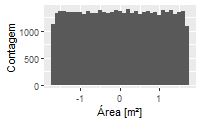
\includegraphics[width=\linewidth]{zscore_plot_area.png}
	\end{minipage}%
	\begin{minipage}{.33\textwidth}
		\centering
		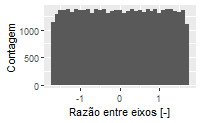
\includegraphics[width=\linewidth]{zscore_plot_ratio.png}
	\end{minipage}%
	\begin{minipage}{.33\textwidth}
		\centering
		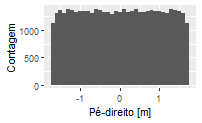
\includegraphics[width=\linewidth]{zscore_plot_height.png}
	\end{minipage}
	\centering
	\begin{minipage}{.33\textwidth}
		\centering
		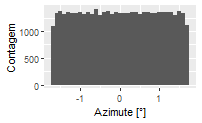
\includegraphics[width=\linewidth]{zscore_plot_azimute.png}
	\end{minipage}%
	\begin{minipage}{.33\textwidth}
		\centering
		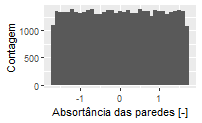
\includegraphics[width=\linewidth]{zscore_plot_abs_wall.png}
	\end{minipage}%
	\begin{minipage}{.33\textwidth}
		\centering
		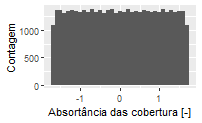
\includegraphics[width=\linewidth]{zscore_plot_abs_roof.png}
	\end{minipage}
	\centering
	\begin{minipage}{.33\textwidth}
		\centering
		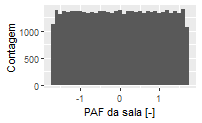
\includegraphics[width=\linewidth]{zscore_plot_wwr_living.png}
	\end{minipage}%
	\begin{minipage}{.33\textwidth}
		\centering
		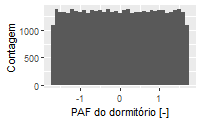
\includegraphics[width=\linewidth]{zscore_plot_wwr_bedroom.png}
	\end{minipage}%
	\begin{minipage}{.33\textwidth}
		\centering
		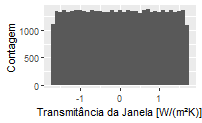
\includegraphics[width=\linewidth]{zscore_plot_window_u.png}
	\end{minipage}
	\centering
	\begin{minipage}{.33\textwidth}
		\centering
		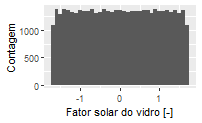
\includegraphics[width=\linewidth]{zscore_plot_shgc.png}
	\end{minipage}%
	\begin{minipage}{.33\textwidth}
		\centering
		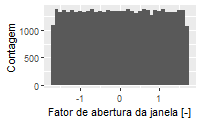
\includegraphics[width=\linewidth]{zscore_plot_open_fac.png}
	\end{minipage}%
	\begin{minipage}{.33\textwidth}
		\centering
		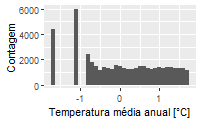
\includegraphics[width=\linewidth]{zscore_plot_DBT.png}
	\end{minipage}
\end{figure}

Os parâmetros \texttt{Parede}, \texttt{Cobertura}, \texttt{Veneziana} e \texttt{Geometria espelhada} foram transformadas em \textit{dummy variables}. Portanto, o parâmetro relacionado aos componentes da parede foi substituído por cinco colunas, o parâmetro relacionado aos componentes da cobertura foi substituído por três colunas, e os parâmetros relacionados à veneziana e à geometria espelhada mantiveram-se com uma coluna.

Com a combinação dos hiperparâmetros do \textit{grid}, 162 modelos foram treinados. 
O tempo total de treinamento foi de 2 horas e 17 minutos.
O modelo escolhido obteve o valor de 0,943 para a média do \textit{cross-validation score}, e teve o processo de treinamento interrompido após 310 iterações. Os hiperparâmetros do modelo escolhido estão apresentados na Tabela \ref{table:bestr2ann}.

\begin{table}[!htb]
	\centering
	\caption{Hiperparâmetros do modelo de \acrshort{ann} final.}
	\label{table:bestr2ann}
	\begin{tabular}{|c |c |}
		\hline
		\textbf{Hiperparâmetro} & \textbf{Valor} \\
		\hline
		\texttt{hidden\_layer\_sizes} & 64 e 128 \\
		\hline
		\texttt{activation} & \texttt{relu} \\
		\hline
		\texttt{batch\_size} & 128 \\
		\hline
		\texttt{learning\_rate\_init} & 0,01 \\
		\hline
		\texttt{tol} & 0,0001 \\
		\hline
	\end{tabular}\\
% 	\small{}
\end{table}

A Figura \ref{fig:scattertrainann} apresenta o gráfico de dispersão comparando os casos preditos com os casos simulados para as amostras de treinamento e de teste. 
A linha pontilhada corresponde à reta \texttt{y = x}, portanto a acurácia nos resultados está relacionada com a proximidade dos pontas à reta. 
Observa-se tendências parecidas em ambos os gráficos, porém a amostra de teste apresenta um número proporcionalmente maior de pontos afastados da reta pontilha. 

\begin{figure}[!htb]
	\caption{Comparação entre predições e valores simulados para as amostras de treino e de teste da \acrshort{ann}.} % of{figure}
	\label{fig:scattertrainann}
	\centering
	\begin{minipage}{.5\textwidth}
		\centering
		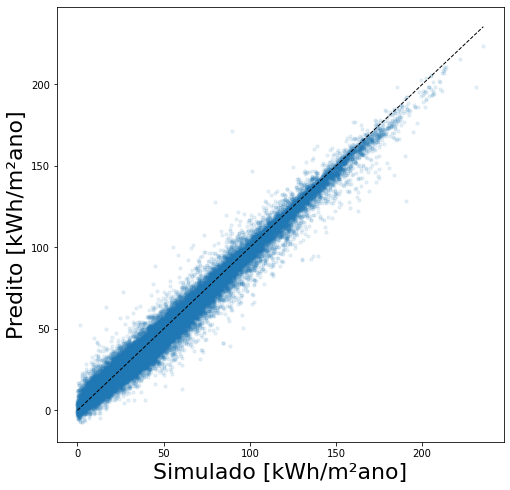
\includegraphics[width=\linewidth]{scatter_train_ann.png}
	\end{minipage}%
	\begin{minipage}{.5\textwidth}
		\centering
		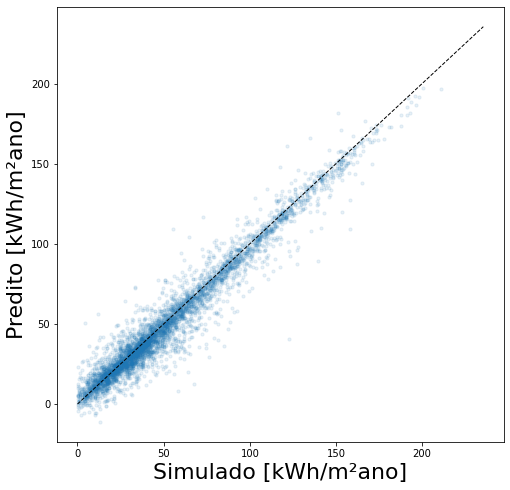
\includegraphics[width=\linewidth]{scatter_test_ann.png}
	\end{minipage}
\end{figure}

Os indicadores de desempenho do metamodelo estão apresentados na Tabela \ref{table:desempenhoann}.
\begin{table}[!htb]
	\centering
	\caption{Indicadores de desempenho do modelo final da \acrshort{ann} para as amostras de treino e de teste.}
	\label{table:desempenhoann}
	\begin{tabular}{|c |c |c |}
		\hline
		\textbf{Indicador} & \textbf{Treino} & \textbf{Teste} \\
		\hline
		\acrshort{r2} & 0,975 & 0,945 \\
		\hline
		\acrshort{rmse} & 5,97 & 8.76 \\
		\hline
		MAE & 4,29 & 5.92 \\
		\hline
		\acrshort{ae95} & 12,05 & 18.85 \\
		\hline
	\end{tabular}\\
% 	\small{}
\end{table}

\subsection{\textit{Gradient Boosting Machine}}
%%%%%%%%%%%%%%%%%%%%%%%%%%%%%%%%%%%%%%%%%%%%%%%%%%%%%%%%%%%%%%%%%

Com a combinação dos hiperparâmetros do \textit{grid}, 243 modelos foram treinados pelo GBM.
O tempo total de treinamento foi de 17 horas e 1 minuto.
O modelo escolhido obteve o valor de 0,991 para a média do \textit{cross-validation score}. Os hiperparâmetros do modelo escolhido estão apresentados na Tabela \ref{table:bestr2}.

\begin{table}[!htb]
	\centering
	\caption{Hiperparâmetros do modelo final de GBM.}
	\label{table:bestr2}
	\begin{tabular}{|c |c |}
		\hline
		\textbf{Hiperparâmetro} & \textbf{Valor} \\
		\hline
		\texttt{n\_estimators} & 40.000 \\
		\hline
		\texttt{max\_depth} & 5 \\
		\hline
		\texttt{min\_samples\_split} & 100 \\
		\hline
		\texttt{loss} & \texttt{huber} \\
		\hline
		\texttt{learning\_rate} & 0,05 \\
		\hline
	\end{tabular}\\
% 	\small{}
\end{table}

A Figura \ref{fig:scattertrain} apresenta o gráfico de dispersão comparando os casos preditos com os casos simulados para as amostras de treinamento e de teste. 

\begin{figure}[!htb]
	\caption{Comparação entre predições e valores simulados para as amostras de treino e de teste do GBM.} % of{figure}
	\label{fig:scattertrain}
	\centering
	\begin{minipage}{.5\textwidth}
		\centering
		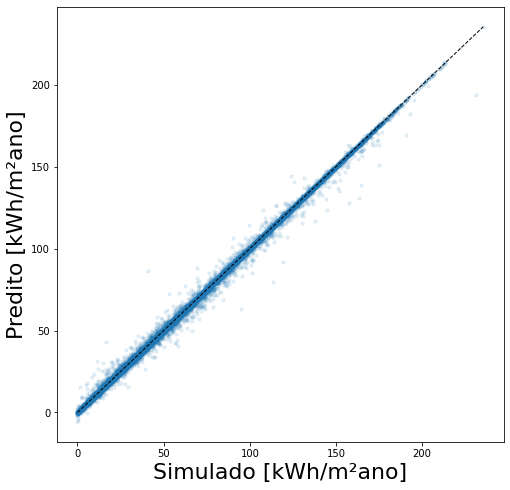
\includegraphics[width=\linewidth]{scatter_train.png}
	\end{minipage}%
	\begin{minipage}{.5\textwidth}
		\centering
		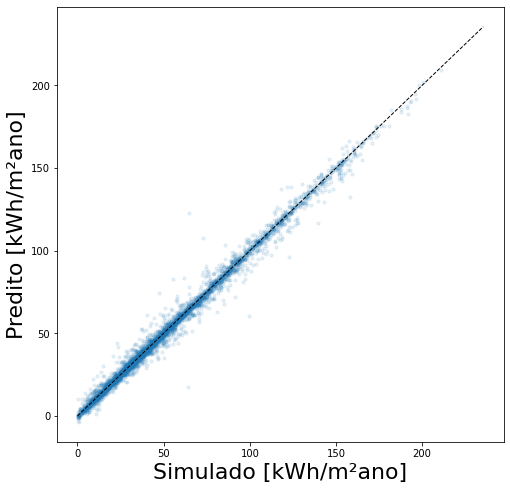
\includegraphics[width=\linewidth]{scatter_test.png}
	\end{minipage}
\end{figure}

Os indicadores de desempenho do metamodelo final estão apresentados na Tabela \ref{table:desempenho}. 

\begin{table}[!htb]
	\centering
	\caption{Indicadores de desempenho do modelo final de GBM para as amostras de treino e de teste. }
	\label{table:desempenho}
	\begin{tabular}{|c |c |c |}
		\hline
		\textbf{Indicador} & \textbf{Treino} & \textbf{Teste} \\
		\hline
		\acrshort{r2} & 0,999 & 0,991 \\
		\hline
		\acrshort{rmse} & 1,17 & 3,48 \\
		\hline
		MAE & 0,48 & 1,97 \\
		\hline
		\acrshort{ae95} & 1,52 & 6,89 \\
		\hline
	\end{tabular}\\
% 	\small{}
\end{table}

\section{Discussão}
%%%%%%%%%%%%%%%%%%%%%%%%%%%%%%%%%%%%%%%%%%%%%%

Apesar de diferenças significativas entre os indicadores de desempenho dos metamodelos avaliados, ambas as abordagens de aprendizado de máquina têm características que podem ser consideradas como mais adequadas, dependendo da maneira como a proposta de desenvolvimento do metamodelo como um todo é determinada.

A primeira diferença que se destaca é a necessidade de pré-processamento dos dados de entrada para a \acrshort{ann}, enquanto que para o GBM não há essa necessidade.
A definição de como será o pré-processamento de cada variável de entrada do metamodelo pode demandar um tempo significativo, pois o tipo de processamento ideal varia de acordo com o tipo de variável.
Neste trabalho utilizou-se apenas a padronização por \textit{z-score} nas variáveis quantitativas, e a transformação das variáveis qualitativas em \textit{dummy variables}, porém existem outros tipos de pré-processamento de dados que podem ser aplicados em diferentes tipos de variáveis.

Outro aspecto que pode ser relevante é o tempo de treinamento dos metamodelos. 
A \acrshort{ann} exigiu um tempo significativamente menor de treinamento (2 horas e 17 minutos) em relação ao GBM (17 horas e 1 minuto).
Considerando-se que o treinamento dos metamodelos foi conduzido em uma máquina com capacidade de processamento e paralelização acima da média, a necessidade de agilidade no desenvolvimento do metamodelo poderia inviabilizar a aplicação do GBM, pois os treinamentos podem demorar mais de 12 horas para finalizar.

Quanto ao desempenho dos metamodelos, o GBM apresentou indicadores consideravelmente melhores do que os da \acrshort{ann}.
Ambos apresentaram valores de \acrshort{r2} aceitáveis, tanto para a amostra de treinamento quanto para a amostra de teste.
A diferença entre os gráficos de dispersão das Figuras \ref{fig:scattertrainann} e \ref{fig:scattertrain} deixa claro como o metamodelo de GBM possui melhor acurácia, com pontos que apresentam-se mais próximos da linha pontilhada, ao longo de toda a faixa de valores de carga térmica considerados.
No caso da \acrshort{ann}, o modelo ainda parece apresentar um enviesamento nas faixas de valores mais altos de carga térmica, fazendo com que o metamodelo subestime o valor de saída nas predições.
Apesar da diferença, em ambos os metamodelos os valores de MAE e \acrshort{rmse} apresentam ordem de grandeza razoável em relação ao parâmetro de saída estimado.
O \acrshort{ae95} também se mantém na mesma ordem de grandeza do MAE e \acrshort{rmse}, o que indica que a acurácia do metamodelo não é comprometida significativamente para pelo menos 95\% dos casos da amostra de teste.

Ambos os metamodelos analisados apresentam indícios de sobreajuste (\textit{overfitting}) dos dados, pois os indicadores obtiveram valores de acurácia inferiores quando medidos a partir da amostra de teste, em relação à amostra de treinamento.
Os motivos que podem causar o \textit{overfitting} diferem entre os métodos de aprendizado de máquina.
No caso da \acrshort{ann}, um número de nós maior que o necessário nas camadas ocultas pode ser o causador, assim como a variável \texttt{tol}, que interfere no número de iterações que ocorrem no processo de treinamento.
No caso do GBM, o aumento no número de estimadores pode causar o fenômeno de sobreajuste, pois após um determinado número de estimadores, há pouca melhora no desempenho do modelo durante o processo de treinamento, momento a partir do qual é possível que o \textit{overfitting} ocorra.
Como o critério de escolha do melhor modelo dentro do \textit{grid} não considera a amostra de teste, é possível que haja modelos com o valor da média do \textit{cross-validation score} próximos aos dos modelos escolhidos, que apresentem desempenho superior para a amostra de teste.
As diferenças entre os indicadores obtidos pela amostra de treino e de teste foram proporcionalmente maiores no caso do GBM, pois seus valores pela amostra de teste apresentaram-se superiores ao dobro dos valores da amostra de treino para o \acrshort{rmse}, MAE e \acrshort{ae95}.
No entanto, como o desempenho do GBM foi significativamente superior em relação à \acrshort{ann}, os indicadores de desempenho da sua amostra de teste obtiveram acurácia significativamente superior aos da amostra de teste utilizando-se a \acrshort{ann}.

\section{Conclusão}

O desenvolvimento de metamodelos pode auxiliar no projeto de edificações, facilitando a estimativa de demanda de carga térmica de ar condicionado. 
Os metamodelos apresentados neste trabalho foram desenvolvidos pelo método de \textit{Gradient Boostin Machine} e \acrlong{ann}, utilizando-se a biblioteca Sklearn, na linguagem de programação Python.

As duas abordagens de aprendizado de máquina apresentadas neste trabalho apresentam características específicas, que podem mostrar-se mais adequadas de acordo com o contexto de aplicação. A \acrshort{ann} exige um pré-processamento de dados, o que pode tornar a sua aplicação mais dificultosa em relação ao GBM, que não exige esse pré-processamento. Por outro lado, o treinamento dos modelos de GBM é significativamente mais custoso computacionalmente, em relação ao treinamento do modelos de \acrshort{ann}.

A utilização de um \textit{grid} permitiu encontrar a melhor combinação de hiperparâmetros para o desenvolvimento dos metamodelos.
Entretanto, esse método define o modelo final sem considerar a amostra de teste, o que pode resultar na ocorrência de sobreajuste (\textit{overfitting}) dos dados.
Em trabalhos futuros, poderia ser explorado um ajuste mais rigoroso dos hiperparâmetros que influenciam no \textit{overfitting}, garantido-se metamodelos mais robustos para casos não vistos.

De acordo com os indicadores de desempenho avaliados (\acrshort{r2},\acrshort{rmse}, MAE e \acrshort{ae95}) os metamodelos foram capazes de estimar as cargas térmicas de ar condicionado adequadamente.
No entanto, o metamodelo de GBM mostrou indicadores consideravelmente superiores em relação ao metamodelo de \acrshort{ann}, tanto para amostra de treino quanto para a amostra de teste.
Portanto, o metamodelo de GBM apresentou-se como o mais adequado para a aplicação proposta neste trabalho.

\bibliographystyle{unsrtnat}  % {plain}
\bibliography{references}
\end{document}
